%% LyX 2.0.5 created this file.  For more info, see http://www.lyx.org/.
%% Do not edit unless you really know what you are doing.
\documentclass[a4paper,danish]{article}
\usepackage[T1]{fontenc}
\usepackage[latin9]{inputenc}
\usepackage{listings}
\usepackage{float}
\usepackage{amsmath}
\usepackage{amssymb}
\usepackage{graphicx}

\makeatletter

%%%%%%%%%%%%%%%%%%%%%%%%%%%%%% LyX specific LaTeX commands.
\pdfpageheight\paperheight
\pdfpagewidth\paperwidth


%%%%%%%%%%%%%%%%%%%%%%%%%%%%%% User specified LaTeX commands.
\usepackage[dot, autosize, outputdir="dotgraphs/"]{dot2texi}
\usepackage{tikz}
\usetikzlibrary{shapes}

\makeatother

\usepackage{babel}
\begin{document}

\title{W1 - Overs�ttere}

\maketitle

\section{Automata Recognising Number Literals}


\subsection{Draw a DFA}

Fra den oprindelige aflevering, havde jeg faktisk en skitse liggende
som jeg tegnede tidligt i processen. Den er identisk med DFA'en som
er udledt i opgave 1.(b-c).

\begin{figure}[H]
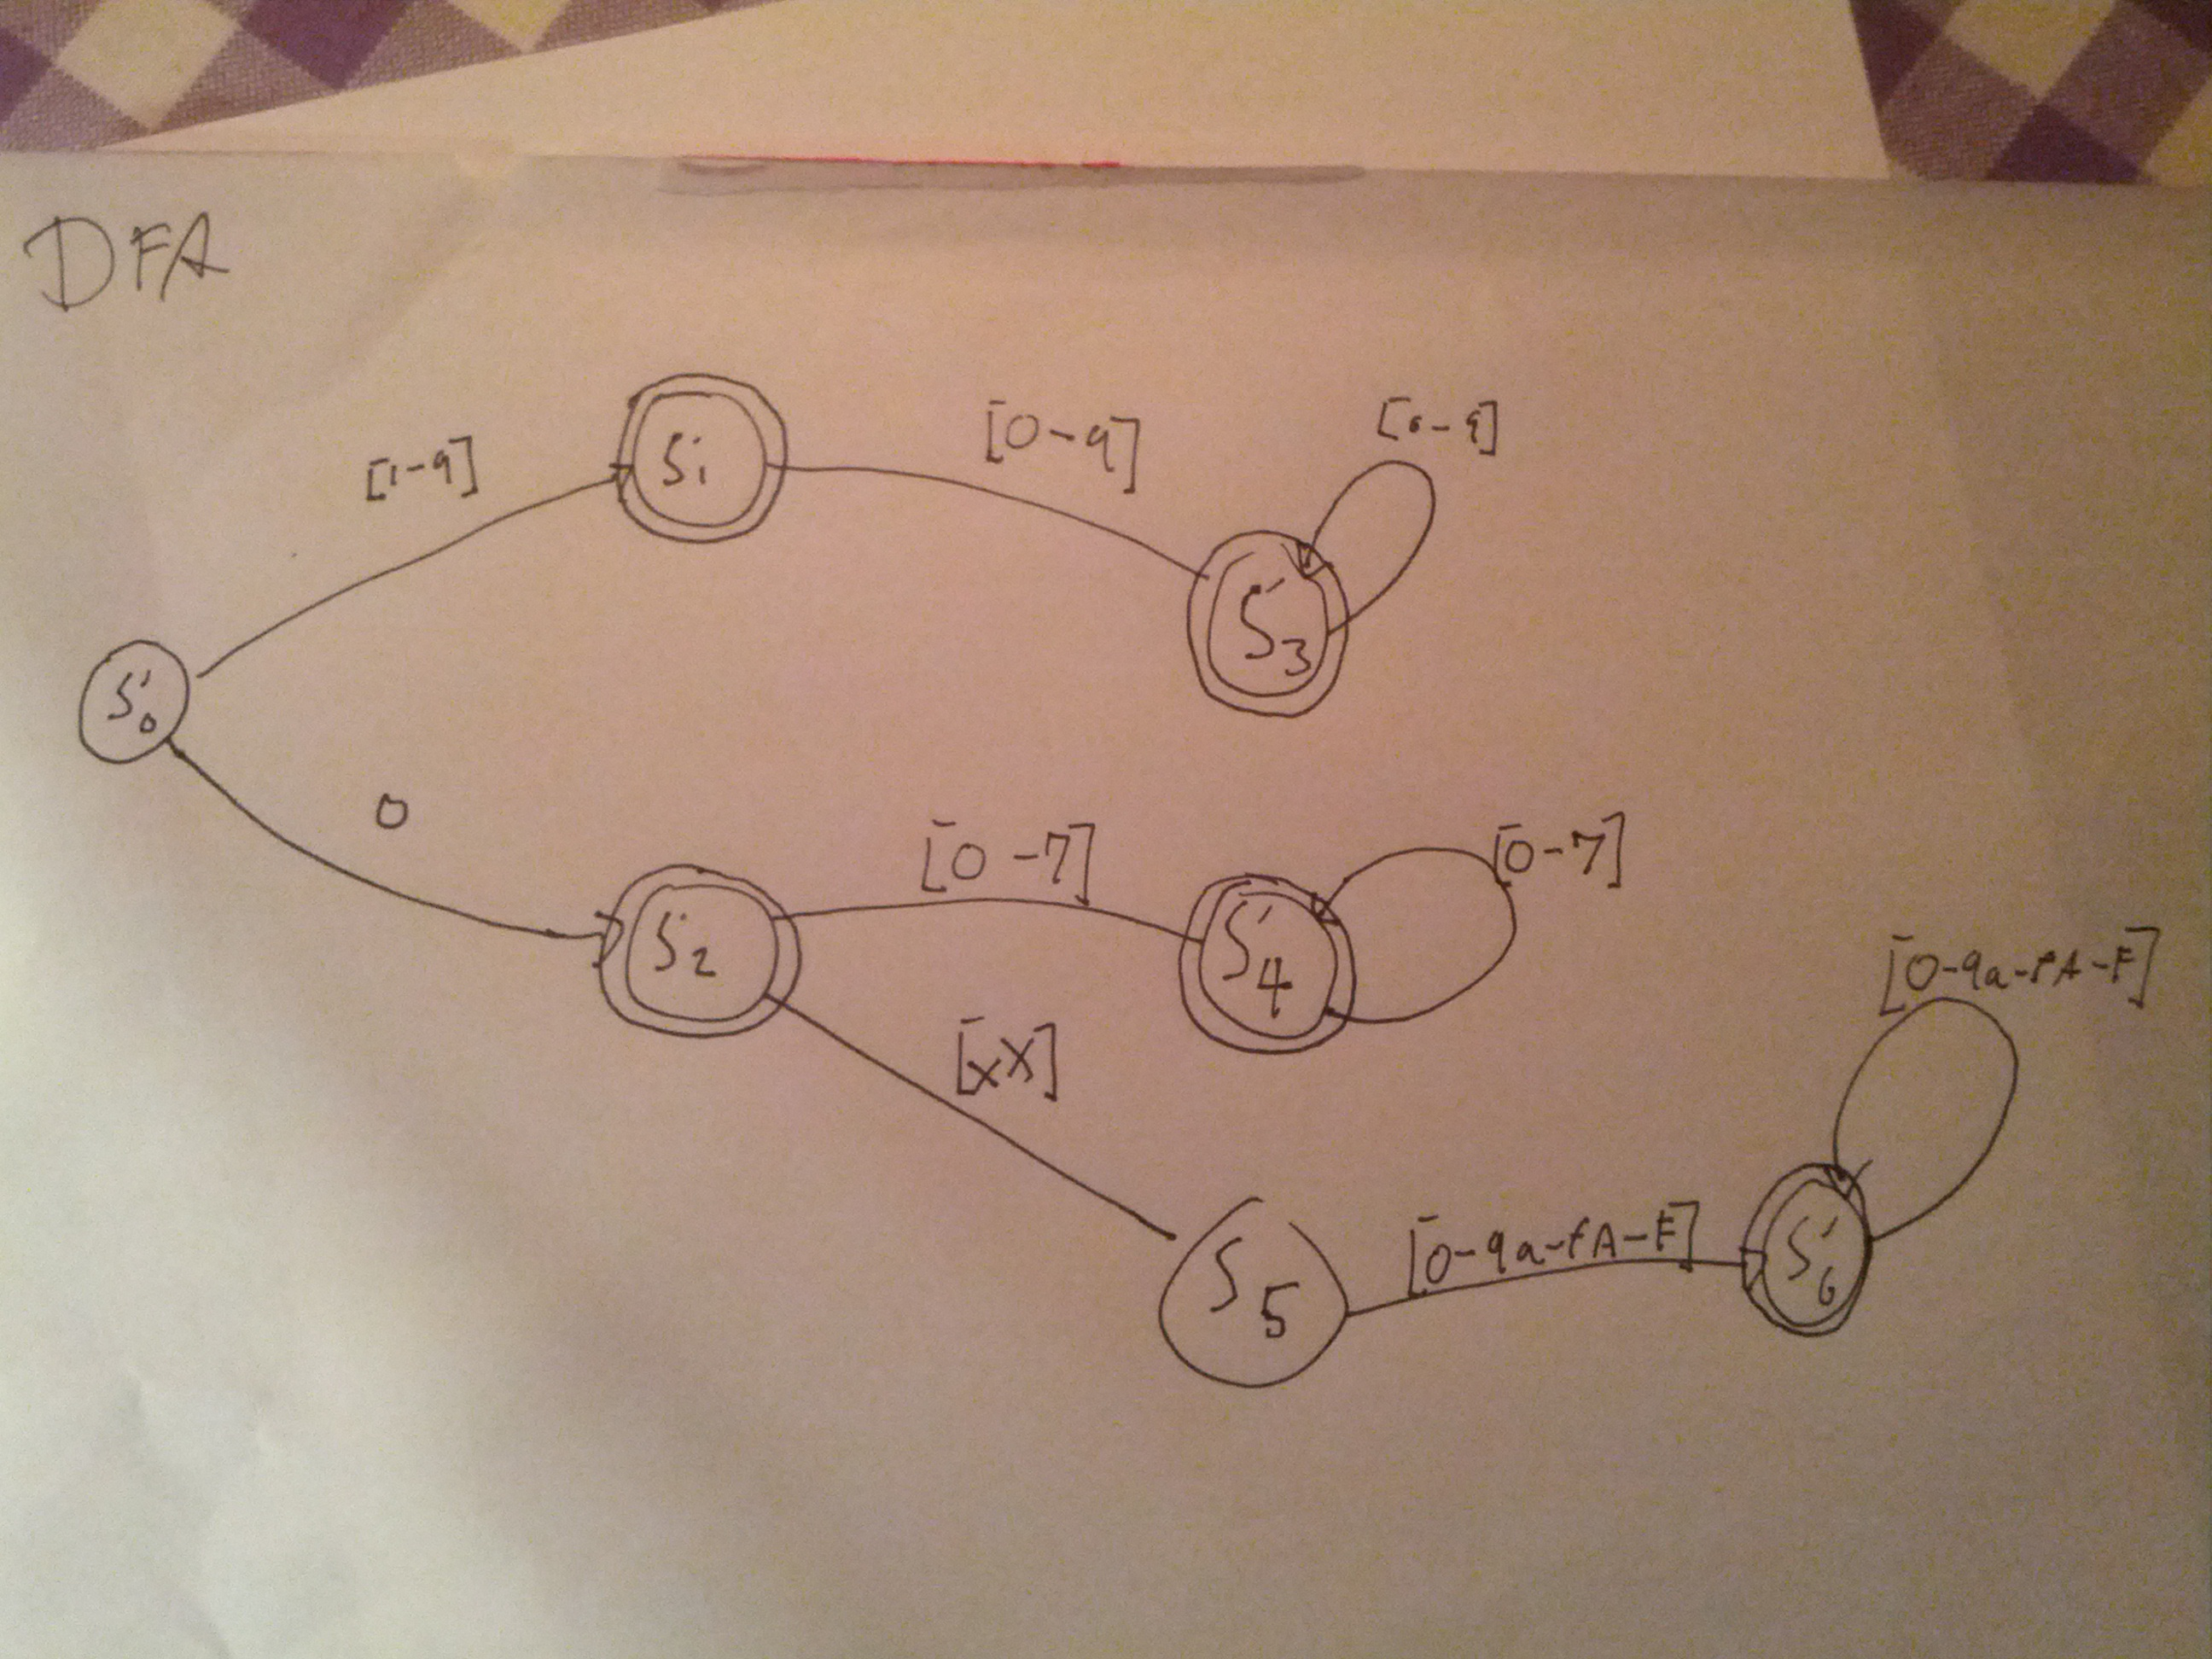
\includegraphics[width=0.95\textwidth]{a1}

\caption{}


\end{figure}



\subsection{Regex to NFA}

Nedenfor ses det regulerer udtryk som konverteres til en NFA.

\texttt{
\[
\mathtt{(([1-9][0-9]*|0)|0([0-7]*|[xX][0-9a-fA-F]+))}
\]
}NFA'en kan ses i Figur 1.

\begin{figure}[H]
\noindent \begin{centering}
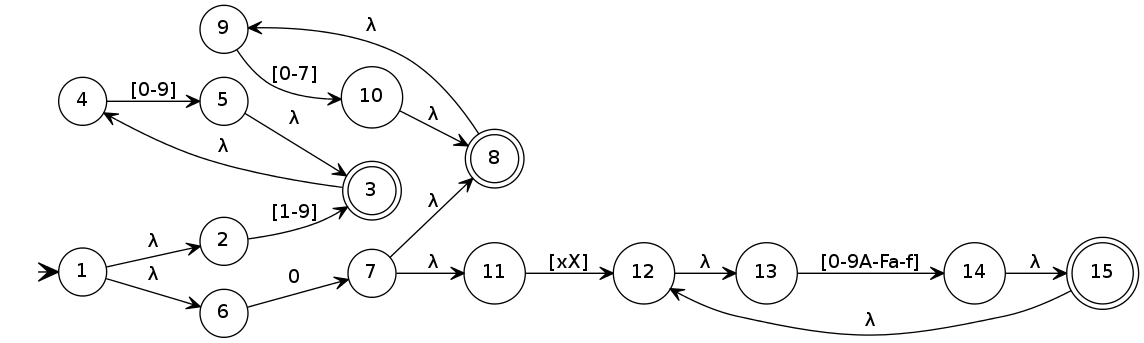
\includegraphics[width=0.8\textheight,angle=90]{1b}
\par\end{centering}

\caption{NFA konstrueret fra det regulerer udtryk ovenfor.}


\end{figure}



\subsection*{1.3 Konvetering til DFA}

\[
\hat{\varepsilon}\{1\}=\{1,2,6\}
\]
$S=\{s'_{0}\}$

\begin{eqnarray*}
move(s'_{0},[1-9]) & = & \hat{\varepsilon}\left(\left\{ t|s\in\left\{ 1,2,6\right\} \textrm{ and }s^{[1-9]}t\in T\right\} \right)\\
 & = & \hat{\varepsilon}(\left\{ 3\right\} )\\
 & = & \{3,4\}\\
 & = & s'_{1}
\end{eqnarray*}


\begin{eqnarray*}
move(s'_{0},0) & = & \hat{\varepsilon}\left(\left\{ t|s\in\left\{ 1,2,6\right\} \textrm{ and }s^{0}t\in T\right\} \right)\\
 & = & \hat{\varepsilon}(\left\{ 7\right\} )\\
 & = & \{7,8,9,11\}\\
 & = & s'_{2}
\end{eqnarray*}
$S=\{\overset{\checkmark}{s'_{0}},s'_{1},s'_{2}\}$

\begin{eqnarray*}
move(s'_{1},[0-9]) & = & \hat{\varepsilon}\left(\left\{ t|s\in\left\{ 3,4\right\} \textrm{ and }s^{[0-9]}t\in T\right\} \right)\\
 & = & \hat{\varepsilon}(\left\{ 5\right\} )\\
 & = & \{3,4,5\}\\
 & = & s'_{3}
\end{eqnarray*}
$S=\{\overset{\checkmark}{s'_{0}},\overset{\checkmark}{s'_{1}},s'_{2},s'_{3}\}$
\begin{eqnarray*}
move(s'_{2},[0-7]) & = & \hat{\varepsilon}\left(\left\{ t|s\in\{7,8,9,11\}\textrm{ and }s^{[0-7]}t\in T\right\} \right)\\
 & = & \hat{\varepsilon}(\left\{ 10\right\} )\\
 & = & \{8,9,10\}\\
 & = & s'_{4}
\end{eqnarray*}


\begin{eqnarray*}
move(s'_{2},\textrm{[Xx]}) & = & \hat{\varepsilon}\left(\left\{ t|s\in\{7,8,9,11\}\textrm{ and }s^{\textrm{[Xx]}}t\in T\right\} \right)\\
 & = & \hat{\varepsilon}(\left\{ 12\right\} )\\
 & = & \{12,13\}\\
 & = & s'_{5}
\end{eqnarray*}
$S=\{\overset{\checkmark}{s'_{0}},\overset{\checkmark}{s'_{1}},\overset{\checkmark}{s'_{2}},s'_{3},s'_{4},s'_{5}\}$
\begin{eqnarray*}
move(s'_{3},[0-9]) & = & \hat{\varepsilon}\left(\left\{ t|s\in\left\{ 3,4,5\right\} \textrm{ and }s^{[0-9]}t\in T\right\} \right)\\
 & = & \hat{\varepsilon}(\left\{ 5\right\} )\\
 & = & \{3,4,5\}\\
 & = & s'_{3}
\end{eqnarray*}
$S=\{\overset{\checkmark}{s'_{0}},\overset{\checkmark}{s'_{1}},\overset{\checkmark}{s'_{2}},\overset{\checkmark}{s'_{3}},s'_{4},s'_{5}\}$

\begin{eqnarray*}
move(s'_{4},[0-7]) & = & \hat{\varepsilon}\left(\left\{ t|s\in\{8,9,10\}\textrm{ and }s^{[0-7]}t\in T\right\} \right)\\
 & = & \hat{\varepsilon}(\left\{ 10\right\} )\\
 & = & \{8,9,10\}\\
 & = & s'_{4}
\end{eqnarray*}
$S=\{\overset{\checkmark}{s'_{0}},\overset{\checkmark}{s'_{1}},\overset{\checkmark}{s'_{2}},\overset{\checkmark}{s'_{3}},\overset{\checkmark}{s'_{4}},s'_{5}\}$

\begin{eqnarray*}
move(s'_{5},\textrm{[0-9a-fA-F]}) & = & \hat{\varepsilon}\left(\left\{ t|s\in\{12,13\}\textrm{ and }s^{\textrm{[0-9a-fA-F]}}t\in T\right\} \right)\\
 & = & \hat{\varepsilon}(\left\{ 14\right\} )\\
 & = & \{12,13,14,15\}\\
 & = & s'_{6}
\end{eqnarray*}
$S=\{\overset{\checkmark}{s'_{0}},\overset{\checkmark}{s'_{1}},\overset{\checkmark}{s'_{2}},\overset{\checkmark}{s'_{3}},\overset{\checkmark}{s'_{4}},\overset{\checkmark}{s'_{5}},s'_{6}\}$

\begin{eqnarray*}
move(s'_{6},\textrm{[0-9a-fA-F]}) & = & \hat{\varepsilon}\left(\left\{ t|s\in\{12,13,14,15\}\textrm{ and }s^{\textrm{[0-9a-fA-F]}}t\in T\right\} \right)\\
 & = & \hat{\varepsilon}(\left\{ 14\right\} )\\
 & = & \{12,13,14,15\}\\
 & = & s'_{6}
\end{eqnarray*}
$S=\{\overset{\checkmark}{s'_{0}},\overset{\checkmark}{s'_{1}},\overset{\checkmark}{s'_{2}},\overset{\checkmark}{s'_{3}},\overset{\checkmark}{s'_{4}},\overset{\checkmark}{s'_{5}},\overset{\checkmark}{s'_{6}}\}$\\
\\
Her er jeg f�rdig og har lavet min DFA med seks states.

\begin{figure}
\noindent \begin{centering}
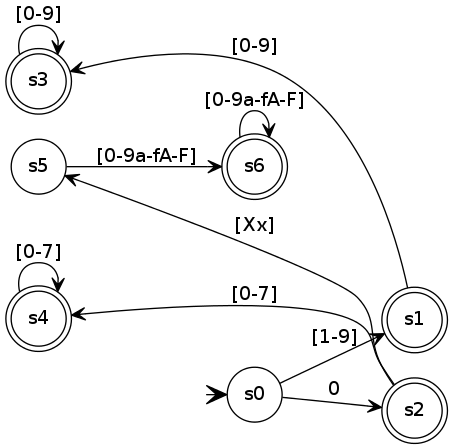
\includegraphics[width=0.75\textwidth]{DFAopg1}
\par\end{centering}

\caption{DFA, konveterert fra NFA i opgave 1.2}


\end{figure}


\cleardoublepage{}\newpage{}


\section{Backtracking Automaton}

\begin{figure}[H]
\noindent \begin{centering}
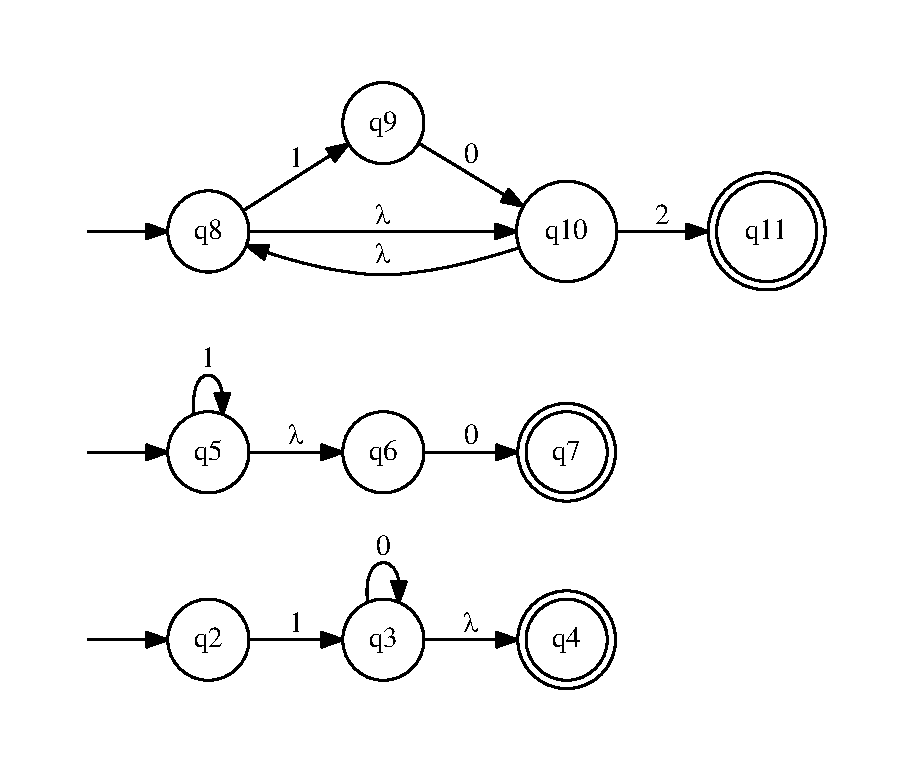
\includegraphics[width=0.75\textwidth]{b1}
\par\end{centering}

\caption{NFA's (before combine) for the three regular expressions given by
the assignment.}
\end{figure}


\begin{figure}[H]
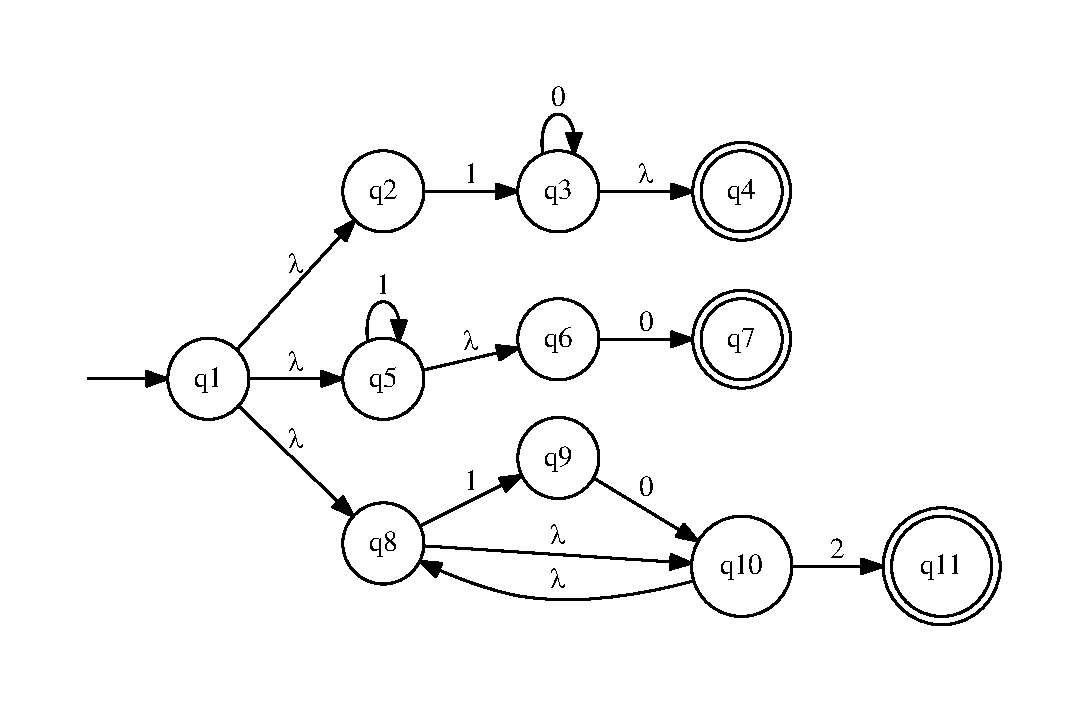
\includegraphics[width=0.9\textwidth]{b2}

\caption{The NFA's from Figure 5 combined to a new single NFA}
\end{figure}



\subsection*{Converting NFA in Figure 5 to DFA}

\begin{minipage}[t]{1\columnwidth}%
\[
\hat{\lambda}\{q1\}=\{q1,q2,q5,q6,q8,q10\}=s'_{0}
\]


\begin{eqnarray*}
move(s'_{0},0) & = & \hat{\lambda}\left(\{q7\}\right)=\{q7\}=s'_{1}\\
move(s'_{0},1) & = & \hat{\lambda}\left(\{q3,q5,q9\}\right)=\{q3,q4,q5,q6,q9\}=s'_{2}\\
move(s'_{0},2) & = & \hat{\lambda}\left(\{q11\}\right)=\{q11\}=s'_{3}\\
\\
move(s'_{2},0) & = & \hat{\lambda}\left(\{q3,q7,q10\}\right)=\{q3,g4,q7,q8,q10\}=s'_{4}\\
move(s'_{2},1) & = & \hat{\lambda}\left(\{q5\}\right)=\{q5,g6\}=s'_{5}\\
\\
move(s'_{4},0) & = & \hat{\lambda}\left(\{q3\}\right)=\{q3,g4\}=s'_{6}\\
move(s'_{4},1) & = & \hat{\lambda}\left(\{q9\}\right)=\{q9\}=s'_{7}\\
move(s'_{4},2) & = & \hat{\lambda}\left(\{q11\}\right)=\{q11\}=s'_{3}\\
\\
move(s'_{5},0) & = & \hat{\lambda}\left(\{q7\}\right)=\{q7\}=s'_{1}\\
move(s'_{5},1) & = & \hat{\lambda}\left(\{q5\}\right)=\{q5,q6\}=s'_{5}\\
\\
move(s'_{6},0) & = & \hat{\lambda}\left(\{q3\}\right)=\{q3,q4\}=s'_{6}\\
\\
move(s'_{7},0) & = & \hat{\lambda}\left(\{q10\}\right)=\{q8,q10\}=s'_{8}\\
\\
move(s'_{8},1) & = & \hat{\lambda}\left(\{q9\}\right)=\{q9\}=s'_{7}\\
move(s'_{8},2) & = & \hat{\lambda}\left(\{q11\}\right)=\{q11\}=s'_{3}
\end{eqnarray*}
%
\end{minipage}
\begin{figure}[H]
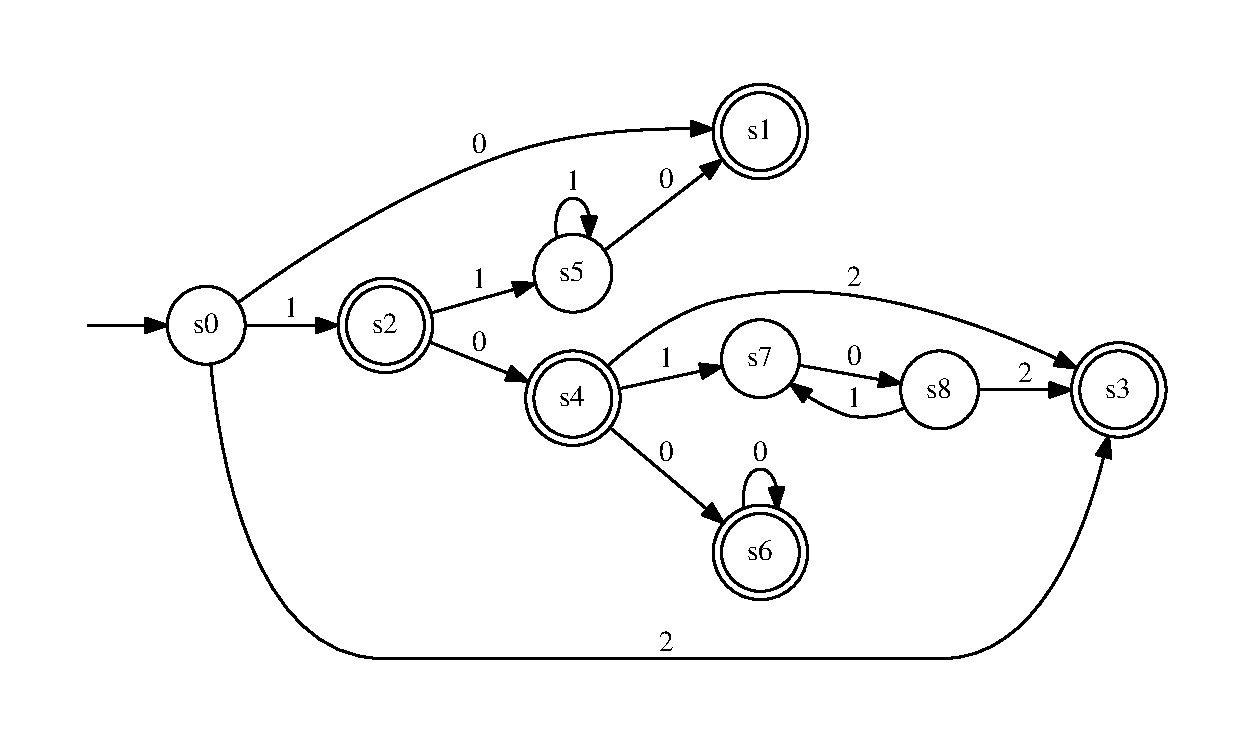
\includegraphics[width=0.9\textwidth]{b3}\caption{}
\end{figure}



\subsection{Transitions and backtracking}

\begin{align*}
_{s_{0}}\;1\;{}_{s_{2}}\;0\;\underset{s_{4}\leftarrow s_{7}}{\underbrace{_{s_{4}}\;1\;{}_{s_{7}}\;0\;{}_{s_{8}}\;1\;{}_{s_{7}}}}\quad|\quad2\quad2\quad1\\
\underline{10}\quad{}_{s_{0}}\;1\;{}_{s_{2}}\;0\;\underset{s_{4}\leftarrow s_{7}}{\underbrace{_{s_{4}}\;1\;{}_{s_{7}}}}\quad|\quad2\quad2\quad1\\
\underline{10}\quad\underline{10}\quad{}_{s_{0}}\;1\;{}_{s_{2}}\quad|\quad2\quad2\quad1\\
\underline{10}\quad\underline{10}\quad\underline{1}\quad{}_{s_{0}}\;2\;{}_{s_{3}}\quad|\quad2\quad1\\
\underline{10}\quad\underline{10}\quad\underline{1}\quad\underline{2}\quad{}_{s_{0}}\;2\;{}_{s_{3}}\quad|\quad1\\
\underline{10}\quad\underline{10}\quad\underline{1}\quad\underline{2}\quad\underline{2}\quad{}_{s_{0}}\;1\;{}_{s_{2}}\quad|\\
\underline{10}\quad\underline{10}\quad\underline{1}\quad\underline{2}\quad\underline{2}\quad\underline{1}
\end{align*}



\section{Lexer i SML}


\subsubsection*{A)}

Regular expresson for the English time format presented in the assignment.

\begin{lstlisting}[basicstyle={\scriptsize\ttfamily},breaklines=true]
((quarter|half) past ([1-9]|10|11|12)|([1-9]|10|11|12) o'clock|([0-9]|[1-5][0-9]) to ([1-9]|10|11|12))
\end{lstlisting}



\subsubsection*{B)}

The solution can be found in the files 3b.lex, 3b.sml and 3b\_test.sml.


\section{More on Regular Languages and Tokenisation}


\subsubsection*{A)}
\begin{enumerate}
\item Ja, da vi leder efter tal der slutter p� 0 eller 5. Noget i den retning
(5|{[}1-9{]}{[}0-9{]}{*}{[}50{]}).
\item Nej. Det vil jeg ikke mene. Vi kan ikke p� den m�de t�lle med regulerer
udtryk.
\item Som du jo pointerede, s� kan man faktisk bare skrive det ud, da vi
arbejder med et en afgr�nset m�nge af heltal.
\begin{lstlisting}[basicstyle={\scriptsize\ttfamily},breaklines=true]
3|4|5|6|7|8|9|12|21|30|33|34|35|36|37|38|39|40|43|44|...|999957|
999958|999959|999960|999963|999964|999965|999966|999967|999968|
999969|999970|999973|999974|999975|999976|999977|999978|999979|
999980|999983|999984|999985|999986|999987|999988|999989|999990|
999993|999994|999995|999996|999997|999998|999999. 
\end{lstlisting}

\end{enumerate}

\subsubsection*{B)}

I Forhold til PL/1 of Fortron s� benytter vi os ikke af lookahead
operatorer, hvilket vil er kr�vet for at kunne parse koden i opgaven.
\end{document}
